%%%%%%%%%%%%%%%%%%%%%%%%%%%%%%%%%%%%%%%%%%%%%%%%%%%%%%%%%%%%%%%%%%%%%%%%%%%%%%%%
\chapter*{Основная часть} % Заголовок
\addcontentsline{toc}{chapter}{Основная часть} % Добавить в оглавление
\refstepcounter{chapter} % Счётчик

%%%%%%%%%%%%%%%%%%%%%%%%%%%%%%%%%%%%%%%%%%%%%%%%%%%%%%%%%%%%%%%%%%%%%%%%%%%%%%%%
%%%%%%%%%%%%%%%%%%%%%%%%%%%%%%%%%%%%%%%%%%%%%%%%%%%%%%%%%%%%%%%%%%%%%%%%%%%%%%%%
\section{Метод полностью параллельной разностной эволюции} \label{s1}

Метод ППРЭ успешно применялся в~различных задачах~\cite{bib3,bib4}.
Совершенствование методов минимизации для нахождения параметров генных 
регуляторных сетей требует наличия набора тестов для оценки новых алгоритмов 
и~реализаций и~сравнения с~предшествующими. 

В самом общем смысле класс рассматриваемых задач можно назвать задачами 
поиска глобального минимума некоторого функционала качества (или функции). 
Способов решения таких задач достаточно много. В работе рассматривается 
модификация стохастического итерационного метода разностной эволюции (РЭ). 
Идея метода РЭ, предложенного Р.~Сторном~\cite{bib1}, заключается в 
моделировании популяции индивидуумов (а точнее, векторов их определяющих). 
Популяция меняется от поколения к поколению, при этом индивидуумы скрещиваются 
и мутируют. 

Метод РЭ имеет набор управляющих параметров (например, размер популяции 
или количество старейших индивидуумов, заменяемых на новые), от которых сильно 
зависит скорость работы и сходимость. Возраст индивидуума — количество итераций,
которые он существует. В~\cite{bibZaharie} была предложена адаптивная схема 
выбора управляющих параметров метода РЭ. В работе~\cite{bibTM} введено 
тригонометрическое преобразование (мутация) вектора-индивидуума, зависящее от 
функционала качества. 

В данной работе рассматривается метод ППРЭ~\cite{bib2,bib5}. Спустя определённое
количество итераций $es\_lambda$ самых старых индивидуумов заменяется 
на~$es\_lambda$ самых «лучших».

\clearpage
%%%%%%%%%%%%%%%%%%%%%%%%%%%%%%%%%%%%%%%%%%%%%%%%%%%%%%%%%%%%%%%%%%%%%%%%%%%%%%%%
%%%%%%%%%%%%%%%%%%%%%%%%%%%%%%%%%%%%%%%%%%%%%%%%%%%%%%%%%%%%%%%%%%%%%%%%%%%%%%%%
\section{Экспериментальные данные (DREAM)} \label{s2}

Проект DREAM предоставляет унифицированные экспериментальные данные для 
тестирования алгоритмов. Каждое «испытание» — некая формализованная задача,
которую предлагается решить независимым группам исследователей. 
Лучшие решения и результаты публикуются. \cite{bib6}. 

В рамках этой работы требуется подобрать близкие к оптимальным значения 
параметров ППРЭ, используя в качестве тестовых задач результаты DREAM6.

%%%%%%%%%%%%%%%%%%%%%%%%%%%%%%%%%%%%%%%%%%%%%%%%%%%%%%%%%%%%%%%%%%%%%%%%%%%%%%%%
\subsection{Постановка задачи} \label{s2_1}

Задача принадлежит области обратной инженерии генных регуляторных сетей. 
Предполагается, что топология генной сети уже определена с достаточным уровнем 
правдоподобия, и теперь требуется охарактеризовать параметры (кинетику) 
этой сети.

Здесь есть два ключевых аспекта, которые требуют внимания: задача оценки 
параметров модели по данной структуре модели, а так же задача проектирования 
наиболее информативных экспериментов для получения неизвестных параметров. 

Итак, даны структуры трёх генных регуляторных сетей, от участников требуется 
разработать и/или применять методы оптимизации, чтобы точно оценить 
параметры моделей, а так же прогнозировать результаты возмущений в этих моделях.

Эти две задачи и являются областью исследования DREAM6. Однако, для тестирования
ППРЭ потребуется рассмотреть лишь первую задачу.

%%%%%%%%%%%%%%%%%%%%%%%%%%%%%%%%%%%%%%%%%%%%%%%%%%%%%%%%%%%%%%%%%%%%%%%%%%%%%%%%
\subsection{Модели генных сетей: Представление данных} \label{s2_2}

Полные структуры генных сетей представлены в формате sbml, tic, и в графическом 
формате. Пример такого представления для первой генной сети приведён на 
рисунке~\ref{img:GrnImage}.

Для каждой сети предоставляется файл (.m) с описанием модели в 
синтаксисе MATLAB. Все переменные помечены в соответствии с их типом. 
Например, переменные, означающие концентрацию белка, помечены как 
$p1$,~$p2$,~...~$p6$. 

Значения каждого символа в генной сети 
объясняются в легенде (рис.~\ref{img:GrnImageDesc}). В скобках перечислены 
префиксы к переменным модели. Линии, соединяющие кодирующую белок 
последовательность с белком, обозначены префиксом «pp». Генерация белка состоит 
из двух логических частей: транскрипция и трансляция. Для простоты эти два 
этапа, изображённые на схеме~\ref{img:GrnImageTT}, не показаны в диаграмме 
генной сети. 

\begin{figure}[h]
  \center{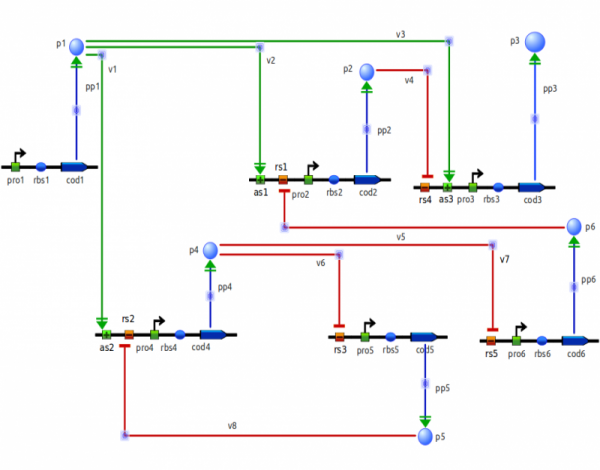
\includegraphics[width=17cm]{model1-600x470.png}}
  \caption{Пример графического представления для первой генной сети}
  \label{img:GrnImage}
\end{figure}

\begin{figure}[h]
  \center{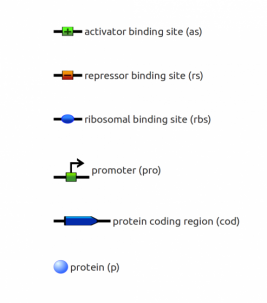
\includegraphics[width=8cm]{diagram_key-267x303.png}}
  \caption{Аннотация к графическому представлению}
  \label{img:GrnImageDesc}
\end{figure}

\begin{figure}[h]
  \center{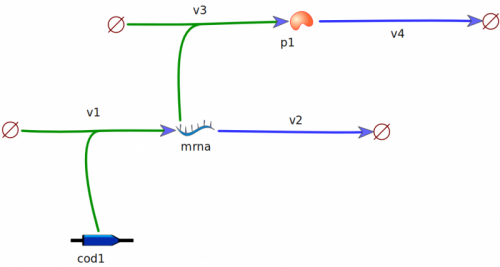
\includegraphics[width=12cm]{protein_production_subfigure-500x267.png}}
  \caption{Транскрипция и трансляция, не показанные на схеме генной сети}
  \label{img:GrnImageTT}
\end{figure}

Имена переменных для концентраций мРНК, результата транскрипции кодирующей 
последовательности имеют соответствующий префикс «pp». Например, переменная, 
соответствующая концентрации мРНК с номером $3$ будет именована как $pp3\_mrna$.

%%%%%%%%%%%%%%%%%%%%%%%%%%%%%%%%%%%%%%%%%%%%%%%%%%%%%%%%%%%%%%%%%%%%%%%%%%%%%%%%
\subsection{Параметры генных сетей} \label{s2_3}

Генная сеть характеризуется топологией (структурой), о которой говорилось выше, 
и набором параметров — скорость трансляции, транскрипции, и параметров, 
отвечающих за сайты связывания рибосом. Если все эти параметры и начальные 
данные (начальные концентрации мРНК, белков) определены, рассматривается 
поведение генной сети на фиксированном интервале времени. Под поведением здесь 
имеется ввиду динамика изменения концентраций мРНК и белка каждого типа.

Таким образом, каждая генная сеть с заданными параметрами порождает ДУ, 
решение которого в конкретном интервале времени пораждает матрицу, 
содержащую набор концентраций для фиксированных моментов времени. В DREAM6 от
участников требуется решить обратную задачу: по данной матрице концентраций 
(пример матрицы~\ref{mRNAtable}) предоставить набор параметров сети.

\clearpage
%%%%%%%%%%%%%%%%%%%%%%%%%%%%%%%%%%%%%%%%%%%%%%%%%%%%%%%%%%%%%%%%%%%%%%%%%%%%%%%%
\subsection{Уравнения генных сетей} \label{s2_3_up}

Все параметры деградации мРНК и белков, имена переменных которых имеют вид: 
$pp\{...\}\_degradation\_rate$ было принято считать одинаковыми в рамках проекта
DREAM. Поэтому в ДУ для моделей я обозначил все эти параметры как 
$degradation\_rate$. 

Система ДУ для модели 1:
\[ \begin{aligned}
  \frac{d}{dt}&[pp1\_mrna] = pro1\_strength - [pp1\_mrna]; \\
  \frac{d}{dt}&[pp2\_mrna] = pro2\_strength
    \cdot \frac{(\frac{[p1]}{v2\_Kd})^{v2\_h}}{1+(\frac{[p1]}{v2\_Kd})^{v2\_h}}
    \cdot \frac{1}{1+(\frac{[p6]}{v5\_Kd})^{v5\_h}} \\
    & \cdot degradation\_rate - [pp2\_mrna]; \\
  \frac{d}{dt}&[pp3\_mrna] = pro3\_strength 
    \cdot \frac{(\frac{[p1]}{v3\_Kd})^{v2\_h}}{1+(\frac{[p1]}{v3\_Kd})^{v3\_h}} 
    \cdot \frac{1}{1+(\frac{[p2]}{v4\_Kd})^{v4\_h}} \\
    & \cdot degradation\_rate - [pp3\_mrna]; \\
  \frac{d}{dt}&[pp4\_mrna] = pro4\_strength 
    \cdot \frac{(\frac{[p1]}{v1\_Kd})^{v2\_h}}{1+(\frac{[p1]}{v1\_Kd})^{v1\_h}} 
    \cdot \frac{1}{1+(\frac{[p5]}{v8\_Kd})^{v8\_h}} \\
    & \cdot degradation\_rate - [pp4\_mrna]; \\
  \frac{d}{dt}&[pp5\_mrna] = pro5\_strength
    \cdot \frac{1}{1+(\frac{[p4]}{v6\_Kd})^{v6\_h}} \cdot degradation\_rate \\
    & - [pp5\_mrna]; \\
  \frac{d}{dt}&[pp6\_mrna] = pro6\_strength
    \cdot \frac{1}{1+(\frac{[p4]}{v7\_Kd})^{v7\_h}} \cdot degradation\_rate \\
    & - [pp6\_mrna]; \\
  \frac{d}{dt}&[p1] = rbs1\_strength \cdot [pp1\_mrna] - degradation\_rate \cdot [p1]; \\
  \frac{d}{dt}&[p2] = rbs2\_strength \cdot [pp2\_mrna] - degradation\_rate \cdot [p2]; \\
  \frac{d}{dt}&[p3] = rbs3\_strength \cdot [pp3\_mrna] - degradation\_rate \cdot [p3]; \\
  \frac{d}{dt}&[p4] = rbs4\_strength \cdot [pp4\_mrna] - degradation\_rate \cdot [p4]; \\
  \frac{d}{dt}&[p5] = rbs5\_strength \cdot [pp5\_mrna] - degradation\_rate \cdot [p5]; \\
  \frac{d}{dt}&[p6] = rbs6\_strength \cdot [pp6\_mrna] - degradation\_rate \cdot [p6];
\end{aligned} \]

Система ДУ для модели 2:
\[ \begin{aligned}
  \frac{d}{dt}&[pp1\_mrna] = pro1\_strength - degradation\_rate \cdot [pp1\_mrna]; \\
  \frac{d}{dt}&[pp2\_mrna] = pro2\_strength 
    \cdot \biggl(\frac{(\frac{[p1]}{v1\_Kd})^{v1\_h}}{1+(\frac{[p1]}{v1\_Kd})^{v1\_h}} + 
    \frac{(\frac{[p2]}{v3\_Kd})^{v3\_h}}{1+(\frac{[p2]}{v3\_Kd})^{v3\_h}}\biggr) \\ 
    & - degradation\_rate \cdot [pp2\_mrna]; \\
  \frac{d}{dt}&[pp3\_mrna] = pro3\_strength 
    \cdot \biggl(\frac{(\frac{[p1]}{v9\_Kd})^{v9\_h}}{1+(\frac{[p1]}{v9\_Kd})^{v9\_h}} + 
    \frac{(\frac{[p2]}{v10\_Kd})^{v10\_h}}{1+(\frac{[p2]}{v10\_Kd})^{v10\_h}}\biggr) \\
    & - degradation\_rate \cdot [pp3\_mrna]; \\
  \frac{d}{dt}&[pp4\_mrna] = pro4\_strength 
    \cdot \frac{1}{1+(\frac{[p3]}{v2\_Kd})^{v2\_h}} \\
    & - degradation\_rate \cdot [pp4\_mrna]; \\
  \frac{d}{dt}&[pp5\_mrna] = pro5\_strength 
    \cdot \frac{(\frac{[p2]}{v4\_Kd })^{v4\_h }}{1+(\frac{[p2]}{v4\_Kd })^{v4\_h }} 
    \cdot \frac{1}{1+(\frac{[p5]}{v5\_Kd})^{v5\_h}} \\
    & - degradation\_rate \cdot [pp5\_mrna]; \\
  \frac{d}{dt}&[pp6\_mrna] = pro6\_strength 
    \cdot \frac{1}{1+(\frac{[p4]}{v6\_Kd})^{v6\_h}} \\
    & - degradation\_rate \cdot [pp6\_mrna]; \\
  \frac{d}{dt}&[pp7\_mrna] = pro7\_strength 
    \cdot \frac{(\frac{[p7]}{v8\_Kd })^{v8\_h }}{1+(\frac{[p7]}{v8\_Kd })^{v8\_h }} 
    \cdot \frac{1}{1+(\frac{[p6]}{v7\_Kd})^{v7\_h}} \\ 
    & - degradation\_rate \cdot [pp7\_mrna]; \\
  \frac{d}{dt}&[p1] = rbs1\_strength \cdot [pp1\_mrna] - degradation\_rate \cdot [p1]; \\
  \frac{d}{dt}&[p2] = rbs2\_strength \cdot [pp2\_mrna] - degradation\_rate \cdot [p2]; \\
  \frac{d}{dt}&[p3] = rbs3\_strength \cdot [pp3\_mrna] - degradation\_rate \cdot [p3]; \\
  \frac{d}{dt}&[p4] = rbs4\_strength \cdot [pp4\_mrna] - degradation\_rate \cdot [p4]; \\
  \frac{d}{dt}&[p5] = rbs5\_strength \cdot [pp5\_mrna] - degradation\_rate \cdot [p5]; \\
  \frac{d}{dt}&[p6] = rbs6\_strength \cdot [pp6\_mrna] - degradation\_rate \cdot [p6]; \\
  \frac{d}{dt}&[p7] = rbs7\_strength \cdot [pp7\_mrna] - degradation\_rate \cdot [p7]; \\
\end{aligned} \]

Система ДУ для модели 3:
\[ \begin{aligned}
  \frac{d}{dt}&[pp1\_mrna] = pro1\_strength - degradation\_rate \cdot [pp1\_mrna]; \\
  \frac{d}{dt}&[pp2\_mrna] = pro2\_strength \cdot 
    \biggl(\frac{(\frac{[p1]}{v1\_Kd})^{v1\_h}}{1+(\frac{[p1]}{v1\_Kd})^{v1\_h}} 
    \cdot \frac{1}{1+(\frac{[p9]}{v13\_Kd})^{v13\_h}}\biggr) \\
    & - degradation\_rate \cdot [pp2\_mrna]; \\
  \frac{d}{dt}&[pp3\_mrna] = pro3\_strength \cdot 
    \biggl(\frac{1}{1+(\frac{[p2]}{v2\_Kd})^{v2\_h}} 
    \cdot \frac{1}{1+(\frac{[p3]}{v3\_Kd})^{v3\_h}}\biggr) \\
    & - degradation\_rate \cdot [pp3\_mrna]; \\
  \frac{d}{dt}&[pp4\_mrna] = pro4\_strength \cdot 
    \biggl(\frac{1}{1+(\frac{[p3]}{v15\_Kd})^{v15\_h}} 
    \cdot \frac{1}{1+(\frac{[p2]}{v14\_Kd})^{v14\_h}}\biggr) \\
    & - degradation\_rate \cdot [pp4\_mrna]; \\
  \frac{d}{dt}&[pp5\_mrna] = pro5\_strength 
    \cdot \frac{(\frac{[p4]}{v4\_Kd})^{v4\_h}}{1+(\frac{[p4]}{v4\_Kd})^{v4\_h}} \\
    & - degradation\_rate \cdot [pp5\_mrna]; \\
  \frac{d}{dt}&[pp6\_mrna] = pro6\_strength \cdot 
    \biggl(\frac{(\frac{[p5]}{v5\_Kd})^{v5\_h}}{1+(\frac{[p5]}{v5\_Kd})^{v5\_h}} + 
    \frac{(\frac{[p6]}{v6\_Kd})^{v6\_h}}{1+(\frac{[p6]}{v6\_Kd})^{v6\_h}}\biggr) \\
    & - degradation\_rate \cdot [pp6\_mrna]; \\
  \frac{d}{dt}&[pp7\_mrna] = pro7\_strength \cdot 
    \biggl(\frac{(\frac{[p6]}{v8\_Kd})^{v8\_h}}{1+(\frac{[p6]}{v8\_Kd})^{v8\_h}} + 
    \frac{(\frac{[p5]}{v9\_Kd})^{v9\_h}}{1+(\frac{[p5]}{v9\_Kd})^{v9\_h}}\biggr) \\
    & - degradation\_rate \cdot [pp7\_mrna]; \\
  \frac{d}{dt}&[pp8\_mrna] = pro8\_strength \cdot 
    \biggl(\frac{(\frac{[p7]}{v7\_Kd})^{v7\_h}}{1+(\frac{[p7]}{v7\_Kd})^{v7\_h}} 
    \cdot \frac{1}{1+(\frac{[p8]}{v11\_Kd})^{v11\_h}}\biggr) \\
    & - degradation\_rate \cdot [pp8\_mrna]; \\
  \frac{d}{dt}&[pp9\_mrna] = pro9\_strength \cdot 
    \biggl(\frac{(\frac{[p7]}{v10\_Kd})^{v10\_h}}{1+(\frac{[p7]}{v10\_Kd})^{v10\_h}} 
    \cdot \frac{1}{1+(\frac{[p8]}{v12\_Kd})^{v12\_h}}\biggr) \\
    & - degradation\_rate \cdot [pp9\_mrna]; \\
  \frac{d}{dt}&[p\{i\}] = rbs\{i\}\_strength \cdot [pp\{i\}\_mrna] - degradation\_rate \cdot [p\{i\}]; \\
\end{aligned} \]

Для $\{i\} = 1, \dots, 9$.

%%%%%%%%%%%%%%%%%%%%%%%%%%%%%%%%%%%%%%%%%%%%%%%%%%%%%%%%%%%%%%%%%%%%%%%%%%%%%%%%
\subsection{Начальные данные и возмущения} \label{s2_4}

Наборы данных, которые предоставляются в качестве входных для оценки параметров,
были сформированы искусственно, путем моделирования, с учётом различных 
возмущений (зашумлений) в генной сети — делеции гена, мРНК нокдаун и изменение 
активности сайтов связывания рибосом. 

Оговорено, что во всех случаях возмущения могут затрагивать только один ген. 
Удаление гена приводит к полной ликвидации как мРНК, так и белка целевого гена. 
В случае миРНК, мРНК деградирует (фиксированное уменьшение в 5 раз), что 
приводит к уменьшению как мРНК, так и концентрации соответствующего белка.

\begin{table}[h]
  \centering
    \begin{tabular}{l|llllll}
        0.0	  & 0.0    & 0.0   & 0.041  & 0.16  & 0.189  & 0.048 \\
        2.0	  & 2.754  & 4.01  & 4.531  & 0.30  & 0.221  & 0.006 \\
        4.0	  & 2.958  & 2.96  & 0.911  & 0.06  & 0.522  & 0.39  \\
        6.0	  & 4.058  & 2.18  & 0.457  & 0.07  & 1.609  & 1.266 \\
        8.0	  & 3.41   & 1.06  & 0.649  & 0.08  & 2.627  & 2.253 \\
        10.0  & 3.459  & 0.68  & 4.398  & 0.07  & 2.979  & 3.811 \\
        12.0  & 2.453  & 0.67  & 6.734  & 0.27  & 2.618  & 2.983 \\
        14.0  & 1.234  & 0.43  & 5.971  & 0.02  & 2.443  & 3.025 \\
        16.0  & 2.385  & 0.43  & 4.606  & 0.0   & 1.821  & 2.823 \\
        18.0  & 3.691  & 0.52  & 5.827  & 0.0   & 3.444  & 2.386 \\
        20.0  & 3.252  & 0.4   & 8.947  & 0.0   & 4.358  & 3.666 
    \end{tabular}
  \caption{Пример таблицы концентраций мРНК для первой генной сети}
  \label{mRNAtable}
\end{table}

\clearpage
%%%%%%%%%%%%%%%%%%%%%%%%%%%%%%%%%%%%%%%%%%%%%%%%%%%%%%%%%%%%%%%%%%%%%%%%%%%%%%%%
%%%%%%%%%%%%%%%%%%%%%%%%%%%%%%%%%%%%%%%%%%%%%%%%%%%%%%%%%%%%%%%%%%%%%%%%%%%%%%%%
\section{Численные эксперименты} \label{s3}

%%%%%%%%%%%%%%%%%%%%%%%%%%%%%%%%%%%%%%%%%%%%%%%%%%%%%%%%%%%%%%%%%%%%%%%%%%%%%%%%
\subsection{Постановка задачи в терминах метода ППРЭ} \label{s3_1}

Метод ППРЭ ищет минимум функционала качества по списку параметров. Параметры — 
неопределённые параметры генной сети, о которых говорилось в предыдущей главе. 

За функционал качества выбирается расстояние между заранее определённой матрицей 
концентраций $W$ (см.~\ref{s2_3}) и матрицей концентраций, полученной с текущими 
параметрами. При этом расстояние понимается как сумма квадратов поэлементных 
разностей двух матриц. 

Как уже было сказано, в качестве оценки работы ППРЭ используются две 
характеристики: 
\begin{enumerate}
	\item Расстояние между известной и полученной матрицами концентраций. Т.е. 
	функционал качества.
	\item Расстояние между известными и полученными параметрами
\end{enumerate}

Более формально: генная сеть, при выборе вектора параметров $p$ и задании
вектора начальных условий $e$ порождает дифференциальное уравнение $ODE(p,e)$. В 
силу однозначности начальных данных, решение этого уравнения единственно. 
Решение — динамика изменений концентраций мРНК и соответствующих им белков. При
фиксированном интервале времени и разбиении решение есть матрица концентраций 
$M^{(p,e)}$.

\[ (p,e) \rightarrow ODE(p,e) \rightarrow M^{(p,e)} \]

Так как вектор начальных условий $e$ неизменен и определён, конструкция 
упрощается:

\[ p \rightarrow ODE(p) \rightarrow M^p \]

Функционал качества для метода ППРЭ есть Евклидово расстояние между матрицами 
концентраций, а $\rho$ есть:

\[ \rho(p,p^*) = \frac{1}{N} \sum\limits_{i = 1}^{N} ln(p_i/p^*_i)^2 \]

Где N — размерность векторов $p$ (текущие параметры) и $p^*$ (известные 
параметры). Теперь каждый вектор параметров $p$ порождает два числа (две 
характеристики, о~которых говорилось выше):

\[ 
p \rightarrow ODE(p) \rightarrow M^p 
\rightarrow \{ \sum\limits_{i,j}(M_{i,j}^p - W_{i,j})^2 , \rho(p,p^*) \}
\]

%%%%%%%%%%%%%%%%%%%%%%%%%%%%%%%%%%%%%%%%%%%%%%%%%%%%%%%%%%%%%%%%%%%%%%%%%%%%%%%%
\subsection{Прогонка управляющих параметров ППРЭ} \label{s3_2}

В качестве критерия остановки было выбрано время, прошедшее с момента начала 
работы. Для каждого запуска выделялось 900 секунд. 

Для всех трёх моделей был зафиксирован параметр $population\_size = 150$ 
($p.size$) и~варьировалось $es\_lambda = 2,15,45$ ($es\_l.$). Всего было 
проведено 12 запусков для каждой модели. 

\begin{table}[h]
\centering
\def\arraystretch{1.5} % отступы
\begin{tabular}{|l|l|llllll|}
\hline % ================================================== %
  \multirow{2}{*}{p.size} & 
  \multirow{2}{*}{es\_l.} & 
  \multicolumn{2}{c|}{Модель 1} & 
  \multicolumn{2}{c|}{Модель 2} & 
  \multicolumn{2}{c|}{Модель 3} \\ \cline{3-8} 
  & & 
  \multicolumn{1}{c|}{Среднее} & 
  \multicolumn{1}{c|}{Мин.} & 
  \multicolumn{1}{c|}{Среднее} & 
  \multicolumn{1}{c|}{Мин.} & 
  \multicolumn{1}{c|}{Среднее} & 
  \multicolumn{1}{c|}{Мин.} \\ 

\hline % ================================================== %
\multirow{3}{*}{150} 
 & 2  & 49.3667 & 25.4139 & 22.8473 & 12.1157 & 48.6207 & 35.7457 \\ \cline{2-2}
 & 15 & 44.0293 & 30.755  & 25.8365 & 12.1114 & 49.8181 & 30.1344 \\ \cline{2-2}
 & 45 & 44.3788 & 24.9287 & 24.1793 & 15.0964 & 44.8327 & 34.6884 \\ 

\hline % ================================================== %
\multicolumn{2}{|l|}{$\Sigma$} & 
\multicolumn{2}{l|}{46.51614} & 
\multicolumn{2}{l|}{20.43136} & 
\multicolumn{2}{l|}{55.38312} \\ 

\hline % ================================================== %
\end{tabular}
\caption{Средние и минимальные значения отклонений модельных концентраций от 
экспериментальных}
\label{contable1}
\end{table}

Здесь $\Sigma$ — значение функционала качества для известных параметров $p^*$.
Динамика изменений $\Sigma$ отражена на графиках:
% \[ \sum\limits_{i,j}(M_{i,j}^{p^*} - W_{i,j})^2 \]

\begin{figure}[h]
  \center{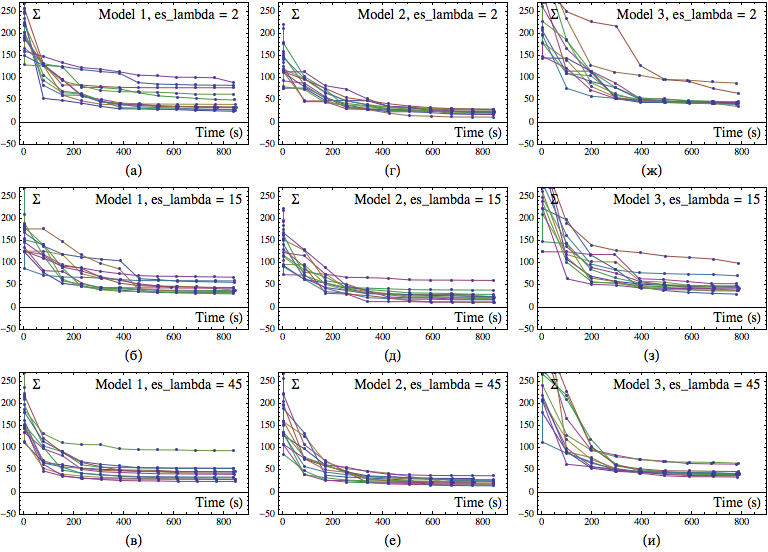
\includegraphics[width=17cm]{p150}}
  \caption{Динамика изменения $\Sigma$. Три модели. 12 независимых запусков. 
  $population\_size = 150$. Модели генных сетей (1,~2,~3), 
  $es\_lambda = 2, 15, 45$.}
  \label{img:p150}
\end{figure}

Из графиков и таблицы очевидно, что в среднем значение минимизируемого 
функционала сходится своему минимальному значению. Кроме того, всегда находился 
набор параметров (вектор $p$, значение $\Sigma$ для которого меньше эталонного).

Рассмотрм изменение расстояния $\rho$ между известными параметрами генной сети 
(предоставленными) и параметрами, найденными методом ППРЭ.

\begin{figure}[h]
  \center{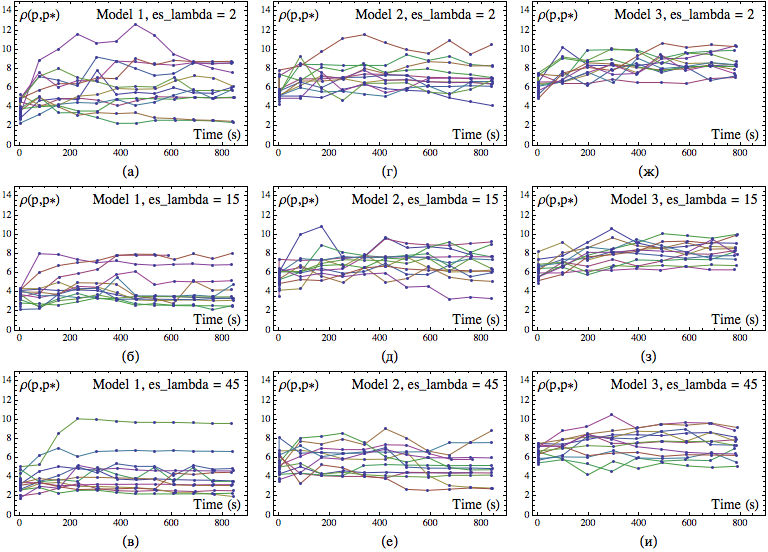
\includegraphics[width=17cm]{p150e}}
  \caption{Динамика изменения $\rho$. Три модели. 12 независимых запусков. 
  $population\_size = 150$. Модели генных сетей (1,~2,~3), 
  $es\_lambda = 2, 15, 45$. }
  \label{img:p150}
\end{figure}

Из графиков видно, что ППРЭ находит не тот вектор, который представлен в 
качестве ответа. Надо полагать, что это происходит из-за большого количества 
параметров ДУ.

Посмотрим, что из себя представляют таблицы концентраций при использовании 
вектора параметров $p$ и $p^*$. Однако, для наглядности рассмотрим не сами 
таблицы $M^p$, а их отличие (разности) от таблицы $W$, т.е. $|M - W|$.

Далее приведены графики модуля разности $|M - W|$, а так же таблицы найденных 
$p_{min}$ и известных $p^*$ параметров, при которых достигается минимум 
функционала:


\begin{table}[h]
  \centering
  \begin{tabular}{|llllll|}
\color[HTML]{909090}0. & \color[HTML]{909090}0. & \color[HTML]{808080}0.041 & \color[HTML]{606060}0.166 & \color[HTML]{505050}0.189 & \color[HTML]{808080}0.048 \\ 
\color[HTML]{606060}0.16 & \color[HTML]{707070}0.093 & \color[HTML]{000000}0.94 & \color[HTML]{606060}0.15 & \color[HTML]{909090}0.02 & \color[HTML]{404040}0.235 \\ 
\color[HTML]{909090}0.013 & \color[HTML]{808080}0.035 & \color[HTML]{707070}0.103 & \color[HTML]{808080}0.035 & \color[HTML]{000000}0.563 & \color[HTML]{000000}0.695 \\ 
\color[HTML]{000000}1.065 & \color[HTML]{000000}0.874 & \color[HTML]{000000}1.204 & \color[HTML]{808080}0.074 & \color[HTML]{000000}0.852 & \color[HTML]{000000}1.195 \\ 
\color[HTML]{101010}0.411 & \color[HTML]{202020}0.366 & \color[HTML]{000000}3.889 & \color[HTML]{707070}0.087 & \color[HTML]{303030}0.286 & \color[HTML]{000000}0.66 \\ 
\color[HTML]{000000}0.459 & \color[HTML]{606060}0.142 & \color[HTML]{000000}1.301 & \color[HTML]{808080}0.073 & \color[HTML]{909090}0.009 & \color[HTML]{000000}0.823 \\ 
\color[HTML]{000000}0.547 & \color[HTML]{606060}0.173 & \color[HTML]{000000}0.807 & \color[HTML]{303030}0.277 & \color[HTML]{101010}0.38 & \color[HTML]{909090}0.015 \\ 
\color[HTML]{000000}1.766 & \color[HTML]{808080}0.067 & \color[HTML]{909090}0.003 & \color[HTML]{909090}0.024 & \color[HTML]{000000}0.557 & \color[HTML]{909090}0.025 \\ 
\color[HTML]{000000}0.615 & \color[HTML]{808080}0.065 & \color[HTML]{000000}1.369 & \color[HTML]{909090}0. & \color[HTML]{000000}1.179 & \color[HTML]{505050}0.177 \\ 
\color[HTML]{000000}0.691 & \color[HTML]{808080}0.027 & \color[HTML]{606060}0.15 & \color[HTML]{909090}0. & \color[HTML]{000000}0.444 & \color[HTML]{000000}0.614 \\ 
\color[HTML]{404040}0.252 & \color[HTML]{707070}0.096 & \color[HTML]{000000}2.97 & \color[HTML]{909090}0. & \color[HTML]{000000}1.358 & \color[HTML]{000000}0.666
\end{tabular}

  \caption{Модель 1. Таблица концентраций получена параметрами $p^*$, 
  предлагаемыми DREAM6 в качестве ответа. $|W - M^{p^*}|$}
  \label{m1p2}
\end{table}
\begin{table}[h]
  \centering
  \begin{tabular}{|llllll|}
\color[HTML]{909090}0. & \color[HTML]{909090}0. & \color[HTML]{808080}0.041 & \color[HTML]{606060}0.166 & \color[HTML]{505050}0.189 & \color[HTML]{808080}0.048 \\ 
\color[HTML]{606060}0.163 & \color[HTML]{000000}1.119 & \color[HTML]{404040}0.258 & \color[HTML]{606060}0.151 & \color[HTML]{505050}0.221 & \color[HTML]{808080}0.028 \\ 
\color[HTML]{909090}0.017 & \color[HTML]{101010}0.391 & \color[HTML]{707070}0.117 & \color[HTML]{606060}0.127 & \color[HTML]{000000}0.521 & \color[HTML]{909090}0. \\ 
\color[HTML]{000000}1.069 & \color[HTML]{404040}0.258 & \color[HTML]{303030}0.275 & \color[HTML]{909090}0.011 & \color[HTML]{303030}0.307 & \color[HTML]{303030}0.315 \\ 
\color[HTML]{101010}0.415 & \color[HTML]{505050}0.203 & \color[HTML]{505050}0.183 & \color[HTML]{707070}0.075 & \color[HTML]{707070}0.079 & \color[HTML]{404040}0.256 \\ 
\color[HTML]{000000}0.463 & \color[HTML]{707070}0.103 & \color[HTML]{505050}0.193 & \color[HTML]{808080}0.071 & \color[HTML]{606060}0.166 & \color[HTML]{000000}1.009 \\ 
\color[HTML]{000000}0.543 & \color[HTML]{808080}0.034 & \color[HTML]{000000}0.583 & \color[HTML]{303030}0.277 & \color[HTML]{505050}0.209 & \color[HTML]{707070}0.122 \\ 
\color[HTML]{000000}1.762 & \color[HTML]{505050}0.177 & \color[HTML]{000000}0.452 & \color[HTML]{909090}0.024 & \color[HTML]{101010}0.386 & \color[HTML]{606060}0.155 \\ 
\color[HTML]{000000}0.611 & \color[HTML]{606060}0.168 & \color[HTML]{000000}1.86 & \color[HTML]{909090}0. & \color[HTML]{000000}1.009 & \color[HTML]{808080}0.049 \\ 
\color[HTML]{000000}0.695 & \color[HTML]{707070}0.075 & \color[HTML]{000000}0.647 & \color[HTML]{909090}0. & \color[HTML]{000000}0.614 & \color[HTML]{000000}0.486 \\ 
\color[HTML]{404040}0.256 & \color[HTML]{505050}0.197 & \color[HTML]{000000}2.472 & \color[HTML]{909090}0. & \color[HTML]{000000}1.528 & \color[HTML]{000000}0.794
\end{tabular}

  \caption{Модель 1. Таблица концентраций получена подбором параметров 
  $p_{min}$ методом ППРЭ. $|W - M^{p_{min}}|$}
  \label{m1p3}
\end{table}
\begin{figure}[h]
  \begin{minipage}[h]{0.5\linewidth}
    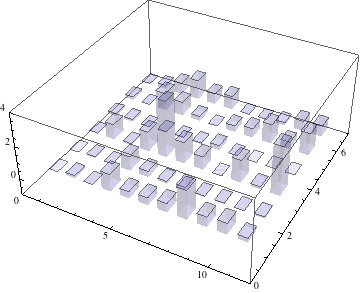
\includegraphics[width=8cm]{tables1f2}
    \caption{График таблицы \ref{m1p2} для $p^*$}
  \end{minipage}
  \hfill
  \begin{minipage}[h]{0.5\linewidth}
    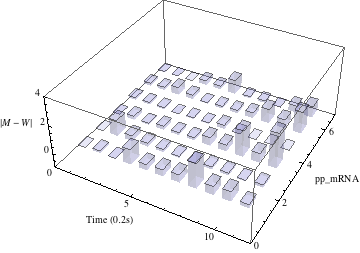
\includegraphics[width=8cm]{tables1f3}
    \caption{График таблицы \ref{m1p3} для $p_{min}$}
  \end{minipage}
\end{figure}


\begin{table}[h]
  \centering
  \begin{tabular}{|lllllll|}
\color[HTML]{909090}0. & \color[HTML]{909090}0. & \color[HTML]{808080}0.044 & \color[HTML]{909090}0. & \color[HTML]{909090}0. & \color[HTML]{707070}0.114 & \color[HTML]{909090}0. \\ 
\color[HTML]{606060}0.132 & \color[HTML]{303030}0.319 & \color[HTML]{505050}0.177 & \color[HTML]{000000}0.896 & \color[HTML]{000000}0.504 & \color[HTML]{404040}0.252 & \color[HTML]{505050}0.219 \\ 
\color[HTML]{707070}0.102 & \color[HTML]{505050}0.187 & \color[HTML]{303030}0.303 & \color[HTML]{606060}0.143 & \color[HTML]{505050}0.176 & \color[HTML]{606060}0.173 & \color[HTML]{000000}1.235 \\ 
\color[HTML]{000000}0.441 & \color[HTML]{000000}1.121 & \color[HTML]{505050}0.2 & \color[HTML]{909090}0.013 & \color[HTML]{909090}0.01 & \color[HTML]{303030}0.288 & \color[HTML]{000000}1.467 \\ 
\color[HTML]{606060}0.152 & \color[HTML]{000000}1.236 & \color[HTML]{101010}0.413 & \color[HTML]{909090}0.003 & \color[HTML]{404040}0.256 & \color[HTML]{000000}1.086 & \color[HTML]{000000}0.444 \\ 
\color[HTML]{606060}0.142 & \color[HTML]{000000}0.434 & \color[HTML]{000000}0.428 & \color[HTML]{808080}0.059 & \color[HTML]{909090}0.011 & \color[HTML]{000000}1.122 & \color[HTML]{707070}0.085 \\ 
\color[HTML]{303030}0.3 & \color[HTML]{000000}0.722 & \color[HTML]{000000}0.979 & \color[HTML]{909090}0. & \color[HTML]{707070}0.119 & \color[HTML]{000000}1.893 & \color[HTML]{909090}0.006 \\ 
\color[HTML]{404040}0.233 & \color[HTML]{101010}0.39 & \color[HTML]{000000}0.739 & \color[HTML]{808080}0.063 & \color[HTML]{000000}0.593 & \color[HTML]{808080}0.052 & \color[HTML]{707070}0.117 \\ 
\color[HTML]{404040}0.251 & \color[HTML]{000000}0.648 & \color[HTML]{404040}0.236 & \color[HTML]{808080}0.063 & \color[HTML]{707070}0.103 & \color[HTML]{404040}0.262 & \color[HTML]{505050}0.203 \\ 
\color[HTML]{808080}0.071 & \color[HTML]{707070}0.097 & \color[HTML]{000000}0.487 & \color[HTML]{606060}0.166 & \color[HTML]{404040}0.264 & \color[HTML]{000000}0.574 & \color[HTML]{909090}0.013 \\ 
\color[HTML]{909090}0.006 & \color[HTML]{000000}0.574 & \color[HTML]{000000}0.886 & \color[HTML]{909090}0.024 & \color[HTML]{808080}0.067 & \color[HTML]{505050}0.213 & \color[HTML]{909090}0.
\end{tabular}

  \caption{Модель 2. Таблица концентраций получена параметрами $p^*$, 
  предлагаемыми DREAM6 в качестве ответа. $|W - M^{p^*}|$}
  \label{m2p2}
\end{table}
\begin{table}[h]
  \centering
  \begin{tabular}{|lllllll|}
\color[HTML]{909090}0. & \color[HTML]{909090}0. & \color[HTML]{808080}0.044 & \color[HTML]{909090}0. & \color[HTML]{909090}0. & \color[HTML]{707070}0.114 & \color[HTML]{909090}0. \\ 
\color[HTML]{808080}0.031 & \color[HTML]{101010}0.388 & \color[HTML]{606060}0.171 & \color[HTML]{000000}0.583 & \color[HTML]{808080}0.027 & \color[HTML]{000000}0.432 & \color[HTML]{404040}0.227 \\ 
\color[HTML]{303030}0.287 & \color[HTML]{000000}0.602 & \color[HTML]{101010}0.401 & \color[HTML]{000000}0.495 & \color[HTML]{505050}0.2 & \color[HTML]{404040}0.263 & \color[HTML]{000000}0.548 \\ 
\color[HTML]{000000}0.629 & \color[HTML]{000000}0.895 & \color[HTML]{000000}0.794 & \color[HTML]{909090}0.004 & \color[HTML]{808080}0.053 & \color[HTML]{606060}0.154 & \color[HTML]{909090}0.005 \\ 
\color[HTML]{808080}0.037 & \color[HTML]{000000}1.08 & \color[HTML]{707070}0.1 & \color[HTML]{808080}0.06 & \color[HTML]{303030}0.295 & \color[HTML]{000000}0.597 & \color[HTML]{303030}0.307 \\ 
\color[HTML]{808080}0.046 & \color[HTML]{000000}0.568 & \color[HTML]{808080}0.056 & \color[HTML]{707070}0.121 & \color[HTML]{808080}0.028 & \color[HTML]{000000}0.662 & \color[HTML]{808080}0.067 \\ 
\color[HTML]{707070}0.112 & \color[HTML]{000000}0.848 & \color[HTML]{000000}0.504 & \color[HTML]{808080}0.061 & \color[HTML]{707070}0.081 & \color[HTML]{000000}1.437 & \color[HTML]{909090}0.009 \\ 
\color[HTML]{808080}0.045 & \color[HTML]{404040}0.266 & \color[HTML]{404040}0.266 & \color[HTML]{909090}0.003 & \color[HTML]{000000}0.555 & \color[HTML]{000000}0.575 & \color[HTML]{707070}0.117 \\ 
\color[HTML]{808080}0.063 & \color[HTML]{000000}0.525 & \color[HTML]{404040}0.236 & \color[HTML]{909090}0.003 & \color[HTML]{808080}0.065 & \color[HTML]{404040}0.248 & \color[HTML]{505050}0.203 \\ 
\color[HTML]{404040}0.259 & \color[HTML]{808080}0.026 & \color[HTML]{909090}0.015 & \color[HTML]{404040}0.226 & \color[HTML]{303030}0.302 & \color[HTML]{808080}0.071 & \color[HTML]{909090}0.013 \\ 
\color[HTML]{505050}0.194 & \color[HTML]{000000}0.697 & \color[HTML]{101010}0.414 & \color[HTML]{808080}0.036 & \color[HTML]{808080}0.029 & \color[HTML]{000000}0.713 & \color[HTML]{909090}0.
\end{tabular}

  \caption{Модель 2. Таблица концентраций получена подбором параметров 
  $p_{min}$ методом ППРЭ. $|W - M^{p_{min}}|$}
  \label{m2p3}
\end{table}
\begin{figure}[h]
  \begin{minipage}[h]{0.5\linewidth}
    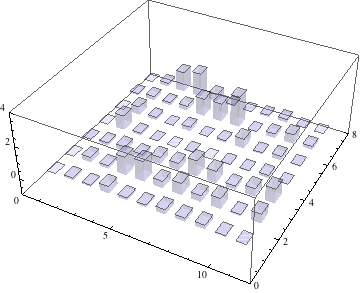
\includegraphics[width=8cm]{tables2f2}
    \caption{График таблицы \ref{m2p2} для $p^*$}
  \end{minipage}
  \hfill
  \begin{minipage}[h]{0.5\linewidth}
    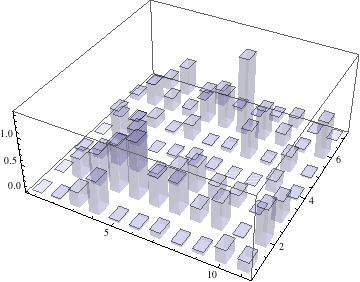
\includegraphics[width=8cm]{tables2f3}
    \caption{График таблицы \ref{m2p3} для $p_{min}$}
  \end{minipage}
\end{figure}


\begin{table}[h]
  \centering
  \begin{tabular}{|lllllllll|}
\color[HTML]{808080}0.072 & \color[HTML]{909090}0. & \color[HTML]{606060}0.127 & \color[HTML]{808080}0.074 & \color[HTML]{909090}0.011 & \color[HTML]{909090}0. & \color[HTML]{909090}0. & \color[HTML]{707070}0.08 & \color[HTML]{909090}0. \\ 
\color[HTML]{505050}0.19 & \color[HTML]{000000}1.026 & \color[HTML]{000000}0.53 & \color[HTML]{000000}0.882 & \color[HTML]{000000}0.636 & \color[HTML]{000000}0.892 & \color[HTML]{000000}1.003 & \color[HTML]{000000}1.472 & \color[HTML]{000000}1.741 \\ 
\color[HTML]{808080}0.052 & \color[HTML]{909090}0.021 & \color[HTML]{000000}3.475 & \color[HTML]{000000}3.462 & \color[HTML]{909090}0.015 & \color[HTML]{707070}0.117 & \color[HTML]{404040}0.258 & \color[HTML]{505050}0.219 & \color[HTML]{000000}0.581 \\ 
\color[HTML]{808080}0.058 & \color[HTML]{909090}0.003 & \color[HTML]{000000}1.552 & \color[HTML]{000000}1.577 & \color[HTML]{707070}0.101 & \color[HTML]{303030}0.305 & \color[HTML]{000000}0.562 & \color[HTML]{909090}0.021 & \color[HTML]{606060}0.158 \\ 
\color[HTML]{000000}0.484 & \color[HTML]{909090}0. & \color[HTML]{000000}0.596 & \color[HTML]{000000}0.534 & \color[HTML]{000000}0.46 & \color[HTML]{000000}1.058 & \color[HTML]{909090}0.018 & \color[HTML]{808080}0.042 & \color[HTML]{909090}0.021 \\ 
\color[HTML]{808080}0.074 & \color[HTML]{707070}0.104 & \color[HTML]{000000}1.045 & \color[HTML]{707070}0.1 & \color[HTML]{000000}1.25 & \color[HTML]{000000}0.668 & \color[HTML]{505050}0.201 & \color[HTML]{606060}0.154 & \color[HTML]{808080}0.066 \\ 
\color[HTML]{404040}0.254 & \color[HTML]{909090}0.01 & \color[HTML]{101010}0.403 & \color[HTML]{000000}0.458 & \color[HTML]{000000}0.486 & \color[HTML]{101010}0.381 & \color[HTML]{000000}0.596 & \color[HTML]{606060}0.146 & \color[HTML]{606060}0.154 \\ 
\color[HTML]{909090}0.013 & \color[HTML]{909090}0.001 & \color[HTML]{000000}0.921 & \color[HTML]{505050}0.217 & \color[HTML]{000000}1.75 & \color[HTML]{808080}0.06 & \color[HTML]{101010}0.389 & \color[HTML]{909090}0.009 & \color[HTML]{808080}0.053 \\ 
\color[HTML]{404040}0.25 & \color[HTML]{808080}0.039 & \color[HTML]{101010}0.416 & \color[HTML]{000000}1.371 & \color[HTML]{000000}1.002 & \color[HTML]{303030}0.311 & \color[HTML]{000000}0.463 & \color[HTML]{606060}0.154 & \color[HTML]{909090}0.016 \\ 
\color[HTML]{000000}0.692 & \color[HTML]{909090}0. & \color[HTML]{101010}0.385 & \color[HTML]{303030}0.317 & \color[HTML]{000000}0.427 & \color[HTML]{000000}0.489 & \color[HTML]{606060}0.147 & \color[HTML]{707070}0.075 & \color[HTML]{707070}0.101 \\ 
\color[HTML]{202020}0.369 & \color[HTML]{707070}0.088 & \color[HTML]{101010}0.42 & \color[HTML]{303030}0.291 & \color[HTML]{404040}0.24 & \color[HTML]{505050}0.193 & \color[HTML]{505050}0.191 & \color[HTML]{808080}0.064 & \color[HTML]{808080}0.06
\end{tabular}

  \caption{Модель 3. Таблица концентраций получена параметрами $p^*$, 
  предлагаемыми DREAM6 в качестве ответа. $|W - M^{p^*}|$}
  \label{m3p2}
\end{table}
\begin{table}[h]
  \centering
  \begin{tabular}{|lllllllll|}
\color[HTML]{808080}0.072 & \color[HTML]{909090}0. & \color[HTML]{606060}0.127 & \color[HTML]{808080}0.074 & \color[HTML]{909090}0.011 & \color[HTML]{909090}0. & \color[HTML]{909090}0. & \color[HTML]{707070}0.08 & \color[HTML]{909090}0. \\ 
\color[HTML]{808080}0.049 & \color[HTML]{909090}0.02 & \color[HTML]{000000}1.397 & \color[HTML]{000000}1.093 & \color[HTML]{000000}0.816 & \color[HTML]{000000}0.432 & \color[HTML]{000000}1.028 & \color[HTML]{000000}1.721 & \color[HTML]{000000}1.602 \\ 
\color[HTML]{505050}0.212 & \color[HTML]{000000}0.755 & \color[HTML]{000000}1.551 & \color[HTML]{000000}0.471 & \color[HTML]{707070}0.102 & \color[HTML]{202020}0.353 & \color[HTML]{808080}0.046 & \color[HTML]{707070}0.081 & \color[HTML]{000000}0.522 \\ 
\color[HTML]{505050}0.221 & \color[HTML]{101010}0.384 & \color[HTML]{000000}0.444 & \color[HTML]{000000}0.486 & \color[HTML]{606060}0.134 & \color[HTML]{707070}0.099 & \color[HTML]{303030}0.288 & \color[HTML]{606060}0.154 & \color[HTML]{606060}0.126 \\ 
\color[HTML]{303030}0.321 & \color[HTML]{404040}0.248 & \color[HTML]{303030}0.301 & \color[HTML]{000000}1.002 & \color[HTML]{000000}0.587 & \color[HTML]{000000}0.856 & \color[HTML]{404040}0.271 & \color[HTML]{505050}0.179 & \color[HTML]{808080}0.06 \\ 
\color[HTML]{707070}0.09 & \color[HTML]{707070}0.111 & \color[HTML]{000000}1.077 & \color[HTML]{606060}0.14 & \color[HTML]{000000}1.424 & \color[HTML]{000000}0.869 & \color[HTML]{000000}0.492 & \color[HTML]{303030}0.291 & \color[HTML]{808080}0.026 \\ 
\color[HTML]{707070}0.091 & \color[HTML]{505050}0.198 & \color[HTML]{000000}0.429 & \color[HTML]{404040}0.248 & \color[HTML]{303030}0.299 & \color[HTML]{505050}0.18 & \color[HTML]{303030}0.304 & \color[HTML]{303030}0.283 & \color[HTML]{707070}0.113 \\ 
\color[HTML]{505050}0.176 & \color[HTML]{505050}0.206 & \color[HTML]{000000}0.959 & \color[HTML]{909090}0.01 & \color[HTML]{000000}1.56 & \color[HTML]{404040}0.261 & \color[HTML]{707070}0.097 & \color[HTML]{606060}0.146 & \color[HTML]{909090}0.012 \\ 
\color[HTML]{101010}0.413 & \color[HTML]{606060}0.168 & \color[HTML]{101010}0.376 & \color[HTML]{000000}1.165 & \color[HTML]{000000}0.811 & \color[HTML]{000000}0.512 & \color[HTML]{000000}0.755 & \color[HTML]{303030}0.291 & \color[HTML]{808080}0.057 \\ 
\color[HTML]{000000}0.529 & \color[HTML]{505050}0.207 & \color[HTML]{202020}0.344 & \color[HTML]{707070}0.111 & \color[HTML]{404040}0.236 & \color[HTML]{303030}0.288 & \color[HTML]{606060}0.145 & \color[HTML]{505050}0.212 & \color[HTML]{808080}0.06 \\ 
\color[HTML]{505050}0.206 & \color[HTML]{707070}0.119 & \color[HTML]{101010}0.379 & \color[HTML]{707070}0.085 & \color[HTML]{808080}0.049 & \color[HTML]{909090}0.008 & \color[HTML]{707070}0.101 & \color[HTML]{505050}0.201 & \color[HTML]{909090}0.019
\end{tabular}

  \caption{Модель 3. Таблица концентраций получена подбором параметров 
  $p_{min}$ методом ППРЭ. $|W - M^{p_{min}}|$}
  \label{m3p3}
\end{table}
\begin{figure}[h]
  \begin{minipage}[h]{0.5\linewidth}
    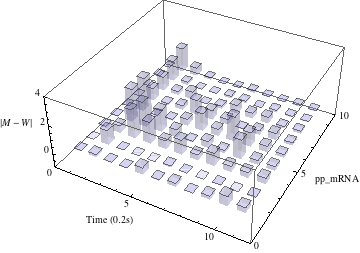
\includegraphics[width=8cm]{tables3f2}
    \caption{График таблицы \ref{m3p2} для $p^*$}
  \end{minipage}
  \hfill
  \begin{minipage}[h]{0.5\linewidth}
    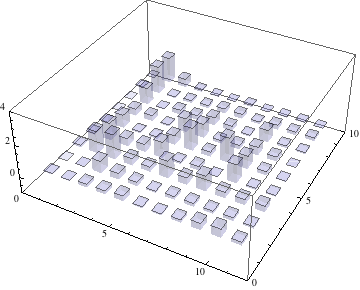
\includegraphics[width=8cm]{tables3f3}
    \caption{График таблицы \ref{m3p3} для $p_{min}$}
  \end{minipage}
\end{figure}


\begin{table}[h]
  \centering
  \begin{tabular}{l|l|lllll}
Параметр & $p^*$ & \multicolumn{5}{c}{$p_{min}$} \\ 
\hline
pro1\_strength & 3 & 2.9963 & 2.92585 & 3.05202 & 3.00715 & 2.91818 \\ 
pro2\_strength & 8 & 3.55804 & 5.93761 & 3.26835 & 3.18463 & 3.70285 \\ 
pro3\_strength & 6 & 6.48589 & 12.998 & 6.33644 & 6.81411 & 13. \\ 
pro4\_strength & 8 & 0.192847 & 0.247468 & 8.29558 & 5.69079 & 1.20639 \\ 
pro5\_strength & 3 & 2.82969 & 2.76794 & 2.72905 & 3.10599 & 2.83064 \\ 
pro6\_strength & 3 & 2.87218 & 3.10766 & 3.1161 & 2.97107 & 2.80903 \\ 
rbs1\_strength & 3.92 & 6.36112 & 12.9358 & 12.9693 & 12.989 & 7.1852 \\ 
rbs2\_strength & 5 & 7.30106 & 7.80092 & 7.32912 & 3.74508 & 1.4508 \\ 
rbs3\_strength & 5 & 11.197 & 13. & 12.9804 & 12.9947 & 12.8981 \\ 
rbs4\_strength & 1 & 0.01 & 0.0191979 & 13. & 11.6184 & 12.1075 \\ 
rbs5\_strength & 5 & 3.58838 & 6.2905 & 12.689 & 5.37672 & 0.0312978 \\ 
rbs6\_strength & 5 & 11.2102 & 12.9964 & 8.33923 & 12.1769 & 13. \\ 
v1\_Kd & 1 & 0.100209 & 6.82445 & 0.55698 & 12.1747 & 12.9971 \\ 
v1\_h & 4 & 9.24381 & 8.37774 & 1.86059 & 6.23978 & 0.0283795 \\ 
v2\_Kd & 1 & 1.2687 & 0.01 & 0.456528 & 1.46449 & 5.16301 \\ 
v2\_h & 2 & 3.05743 & 0.0107374 & 2.52568 & 12.6145 & 7.84212 \\ 
v3\_Kd & 0.1 & 0.981649 & 13. & 0.01 & 0.0242598 & 13. \\ 
v3\_h & 2 & 10.6521 & 0.0100633 & 13. & 4.07633 & 0.01 \\ 
v4\_Kd & 10 & 11.6252 & 13. & 12.9998 & 5.48176 & 1.31392 \\ 
v4\_h & 4 & 6.5367 & 7.68906 & 7.6741 & 3.80357 & 2.16893 \\ 
v5\_Kd & 1 & 10.7801 & 12.9836 & 7.33553 & 12.7475 & 8.96997 \\ 
v5\_h & 1 & 1.46291 & 1.18206 & 1.54623 & 1.61237 & 2.33514 \\ 
v6\_Kd & 0.1 & 0.01 & 0.0100392 & 12.8154 & 1.99358 & 0.01 \\ 
v6\_h & 2 & 8.58302 & 12.0434 & 0.751893 & 0.274631 & 1.03708 \\ 
v7\_Kd & 0.1 & 0.0100073 & 0.0100161 & 1.37711 & 0.402394 & 0.01 \\ 
v7\_h & 2 & 1.3518 & 3.00998 & 1.6421 & 12.6013 & 13. \\ 
v8\_Kd & 0.2 & 0.66476 & 5.63135 & 3.55132 & 2.77787 & 0.01 \\ 
v8\_h & 4 & 7.38939 & 12.8872 & 12.9753 & 8.25712 & 12.8461
\end{tabular}

  \caption{Параметры модели 1}
  \label{m1params}
\end{table}
\begin{table}[h]
  \centering
  \begin{tabular}{l|l|lllll}
Параметр & $p^*$ & \multicolumn{5}{c}{$p_{min}$} \\ 
\hline
pro1\_strength & 1.31 & 1.12166 & 1.3428 & 1.06452 & 1.34043 & 1.18295 \\ 
pro2\_strength & 7.79 & 2.57413 & 2.12451 & 2.16855 & 3.33444 & 3.00753 \\ 
pro3\_strength & 7.79 & 3.63213 & 1.8939 & 1.78388 & 6.27388 & 2.94564 \\ 
pro4\_strength & 4 & 3.66947 & 5.23487 & 11.1304 & 12.067 & 3.59045 \\ 
pro5\_strength & 5.99 & 8.80347 & 8.3395 & 12.7556 & 9.5366 & 4.13528 \\ 
pro6\_strength & 5 & 4.67417 & 4.29806 & 4.56755 & 4.43596 & 4.61987 \\ 
pro7\_strength & 2.93 & 13. & 7.66922 & 5.91811 & 8.94231 & 1.12427 \\ 
rbs1\_strength & 5 & 2.25641 & 10.4715 & 10.2654 & 10.2357 & 3.9725 \\ 
rbs2\_strength & 1 & 9.78127 & 10.119 & 10.4709 & 0.0153719 & 5.27953 \\ 
rbs3\_strength & 5 & 11.8777 & 13. & 6.64263 & 12.2433 & 9.38997 \\ 
rbs4\_strength & 5 & 0.152162 & 12.0366 & 7.55073 & 12.7734 & 2.48847 \\ 
rbs5\_strength & 5 & 2.72958 & 11.4941 & 12.9739 & 0.615125 & 9.13042 \\ 
rbs6\_strength & 5 & 7.72043 & 1.52188 & 12.079 & 12.9991 & 10.7603 \\ 
rbs7\_strength & 5 & 12.9867 & 6.64221 & 11.9133 & 12.9977 & 4.19665 \\ 
v1\_Kd & 10 & 4.86011 & 13. & 8.37926 & 9.51029 & 8.98448 \\ 
v1\_h & 1 & 1.28737 & 4.28145 & 0.0621061 & 11.8475 & 0.0435457 \\ 
v2\_Kd & 2 & 12.998 & 12.9389 & 3.02416 & 6.05854 & 7.13107 \\ 
v2\_h & 2 & 6.0014 & 11.8375 & 12.9628 & 12.947 & 5.50593 \\ 
v3\_Kd & 10 & 1.45081 & 0.01 & 5.63589 & 0.261099 & 10.467 \\ 
v3\_h & 4 & 1.17019 & 12.7148 & 5.37748 & 5.84989 & 0.918297 \\ 
v4\_Kd & 0.001 & 10.4194 & 12.5022 & 10.3433 & 7.53694 & 5.77231 \\ 
v4\_h & 1 & 11.664 & 0.950678 & 1.27285 & 0.248257 & 0.0111751 \\ 
v5\_Kd & 4.951 & 2.60774 & 12.8827 & 12.96 & 12.9668 & 12.9261 \\ 
v5\_h & 4 & 5.50981 & 7.08617 & 12.9986 & 0.166834 & 6.6113 \\ 
v6\_Kd & 0.7093 & 0.01 & 0.580914 & 0.181896 & 0.651964 & 0.070362 \\ 
v6\_h & 2 & 2.73495 & 1.98526 & 1.26195 & 5.05768 & 1.94584 \\ 
v7\_Kd & 1 & 0.0100008 & 0.0568314 & 1.11111 & 0.0181018 & 11.9347 \\ 
v7\_h & 4 & 12.6789 & 13. & 2.88253 & 6.11441 & 6.48009 \\ 
v8\_Kd & 0.01 & 13. & 1.99672 & 13. & 0.0108357 & 0.0100724 \\ 
v8\_h & 4 & 0.01 & 0.0109494 & 1.1386 & 11.0739 & 0.683375 \\ 
v9\_Kd & 10 & 12.9949 & 0.0151922 & 0.0185519 & 6.69634 & 12.8928 \\ 
v9\_h & 1 & 8.5502 & 10.5261 & 0.668325 & 0.39999 & 0.0153574 \\ 
v10\_Kd & 10 & 9.36028 & 13. & 10.9177 & 12.5016 & 12.3133 \\ 
v10\_h & 4 & 12.9581 & 2.40681 & 9.9295 & 11.9624 & 3.31859
\end{tabular}

  \caption{Параметры модели 2}
  \label{m2params}
\end{table}
\begin{table}[h]
  \centering
  \begin{tabular}{l|l|lllll}
Параметр & $p^*$ & \multicolumn{5}{c}{$p_{min}$} \\ 
\hline
pro1\_strength & 2 & 1.83655 & 1.75989 & 1.80524 & 1.70689 & 1.73567 \\ 
pro2\_strength & 4.5077 & 2.73106 & 0.561684 & 0.0141565 & 1.79753 & 10.5839 \\ 
pro3\_strength & 5 & 9.02625 & 7.7042 & 12.9842 & 3.93447 & 12.4497 \\ 
pro4\_strength & 5 & 4.06825 & 3.65868 & 10.0973 & 3.63505 & 12.8847 \\ 
pro5\_strength & 5 & 10.1031 & 5.37787 & 13. & 7.94748 & 11.5807 \\ 
pro6\_strength & 1.31 & 1.20946 & 1.61518 & 1.28631 & 1.29889 & 2.63557 \\ 
pro7\_strength & 1.31 & 3.47279 & 1.87719 & 1.48501 & 1.40278 & 1.20376 \\ 
pro8\_strength & 5 & 0.324542 & 9.94177 & 0.01 & 1.25838 & 6.92487 \\ 
pro9\_strength & 5 & 1.11254 & 9.69905 & 0.01 & 0.130907 & 1.31434 \\ 
rbs1\_strength & 0.3668 & 0.011053 & 0.0125254 & 8.38407 & 0.01 & 0.183802 \\ 
rbs2\_strength & 1.4102 & 12.8511 & 9.12216 & 5.48446 & 0.0628125 & 10.4756 \\ 
rbs3\_strength & 0.8 & 1.754 & 1.1403 & 5.59756 & 0.688286 & 4.00149 \\ 
rbs4\_strength & 2.21 & 12.8869 & 6.68718 & 0.013985 & 9.76812 & 2.21424 \\ 
rbs5\_strength & 0.5 & 0.0100057 & 12.3662 & 9.93452 & 12.8247 & 9.80061 \\ 
rbs6\_strength & 2 & 12.9981 & 11.1952 & 12.6931 & 13. & 0.0509437 \\ 
rbs7\_strength & 5 & 12.6994 & 4.17751 & 0.0145791 & 0.0979573 & 11.0331 \\ 
rbs8\_strength & 3.6377 & 5.18856 & 7.91333 & 6.96911 & 12.981 & 12.2507 \\ 
rbs9\_strength & 8 & 12.9951 & 0.85603 & 3.52368 & 13. & 9.90043 \\ 
v1\_Kd & 11.147 & 1.27036 & 0.158631 & 1.07167 & 10.6224 & 6.26708 \\ 
v1\_h & 1 & 0.605086 & 12.9968 & 0.0878918 & 0.452064 & 2.25854 \\ 
v2\_Kd & 1 & 12.789 & 12.9998 & 0.0220842 & 7.13145 & 11.5336 \\ 
v2\_h & 4 & 2.694 & 0.01 & 6.91033 & 0.71999 & 11.7688 \\ 
v3\_Kd & 20 & 4.12552 & 11.1919 & 12.9999 & 9.79581 & 6.47455 \\ 
v3\_h & 1 & 0.101528 & 12.9759 & 1.94343 & 12.9949 & 1.25699 \\ 
v4\_Kd & 0.2 & 12.9996 & 7.10004 & 12.8009 & 10.006 & 11.9616 \\ 
v4\_h & 4 & 0.0395719 & 12.3663 & 0.0719414 & 0.625118 & 0.412131 \\ 
v5\_Kd & 0.2 & 0.01 & 3.75671 & 12.5781 & 12.0499 & 12.2468 \\ 
v5\_h & 4 & 8.78179 & 13. & 12.3549 & 13. & 10.3321 \\ 
v6\_Kd & 0.04 & 1.14168 & 0.010017 & 2.55974 & 0.0100053 & 12.3909 \\ 
v6\_h & 4 & 4.27492 & 0.0530206 & 10.347 & 12.9636 & 8.99329 \\ 
v7\_Kd & 0.02 & 12.9751 & 10.1405 & 0.101414 & 10.9749 & 0.690458 \\ 
v7\_h & 4 & 9.31997 & 0.0254962 & 10.8923 & 0.541086 & 0.0100963 \\ 
v8\_Kd & 0.04 & 0.01 & 0.967533 & 12.7922 & 9.73419 & 0.01 \\ 
v8\_h & 4 & 0.204643 & 7.1033 & 13. & 12.9828 & 4.52434 \\ 
v9\_Kd & 0.2 & 13. & 10.9287 & 12.9697 & 0.380651 & 12.9955 \\ 
v9\_h & 4 & 6.80736 & 0.0836545 & 12.9986 & 3.16794 & 6.93065 \\ 
v10\_Kd & 0.02 & 9.29614 & 2.99535 & 0.01 & 12.7499 & 12.9959 \\ 
v10\_h & 4 & 0.01 & 0.0552407 & 12.9508 & 0.01 & 4.06318 \\ 
v11\_Kd & 0.1 & 12.7237 & 1.12745 & 2.75496 & 12.7124 & 2.74753 \\ 
v11\_h & 2 & 1.00985 & 13. & 8.59118 & 2.01365 & 2.0733 \\ 
v12\_Kd & 0.1 & 0.01 & 0.24689 & 5.51703 & 5.98262 & 0.0100005 \\ 
v12\_h & 2 & 0.273525 & 9.15347 & 1.67924 & 0.0144777 & 0.279904 \\ 
v13\_Kd & 0.01 & 12.6122 & 10.8823 & 0.0108015 & 4.60434 & 12.9962 \\ 
v13\_h & 2 & 8.16779 & 6.52591 & 3.36257 & 0.364694 & 2.47203 \\ 
v14\_Kd & 1 & 9.14653 & 3.3209 & 0.951031 & 0.0170284 & 3.49404 \\ 
v14\_h & 4 & 11.2696 & 10.1934 & 0.156777 & 13. & 1.30948 \\ 
v15\_Kd & 20 & 13. & 12.7052 & 13. & 12.8918 & 12.3816 \\ 
v15\_h & 1 & 13. & 11.5342 & 0.01 & 13. & 7.19648
\end{tabular}

  \caption{Параметры модели 3}
  \label{m3params}
\end{table}

\clearpage

Была проведена серия экспериментов с изменением параметра, отвечающего 
за способ создания нового поколения ($recombination\_strategy$), 
и фиксированным интервалом времени для каждого запуска. 

Результаты приведены на графике \ref{img:recombination} и в таблице:

\begin{table}[h]
\centering
\def\arraystretch{1.5} % отступы
\begin{tabular}{|l|llllll|}
\hline % ================================================== %
  \multirow{2}{*}{Способ рекомбинации} & 
  \multicolumn{2}{c|}{Модель 1} & 
  \multicolumn{2}{c|}{Модель 2} & 
  \multicolumn{2}{c|}{Модель 3} \\ \cline{2-7} 
  & 
  \multicolumn{1}{c|}{Среднее} & 
  \multicolumn{1}{c|}{Мин.} & 
  \multicolumn{1}{c|}{Среднее} & 
  \multicolumn{1}{c|}{Мин.} & 
  \multicolumn{1}{c|}{Среднее} & 
  \multicolumn{1}{c|}{Мин.} \\ 
\hline % ================================================== %
  de\_3\_bin\_T & 46.0306 & 27.9233 & 30.4181 & 14.1278 & 54.2926 & 32.8514 \\ \cline{1-1}
  de\_3\_bin    & 60.3923 & 33.9588 & 41.1592 & 34.2473 & 76.0278 & 52.8957 \\ \cline{1-1}
  de\_3\_exp\_T & 81.3085 & 44.7055 & 54.6786 & 24.7477 & 81.9631 & 40.2255 \\ \cline{1-1}
  de\_3\_exp    & 77.0761 & 50.8476 & 44.8638 & 30.6153 & 121.066 & 87.7188 \\ \cline{1-1}
  simple        & 98.0068 & 49.9085 & 65.0740 & 36.8293 & 99.6021 & 52.9599 \\
\hline % ================================================== %
  \multicolumn{1}{|l|}{$\Sigma$} & 
  \multicolumn{2}{l|}{46.51614} & 
  \multicolumn{2}{l|}{20.43136} & 
  \multicolumn{2}{l|}{55.38312} \\ 
\hline % ================================================== %
\end{tabular}
\end{table}

\begin{figure}[h]
  \center{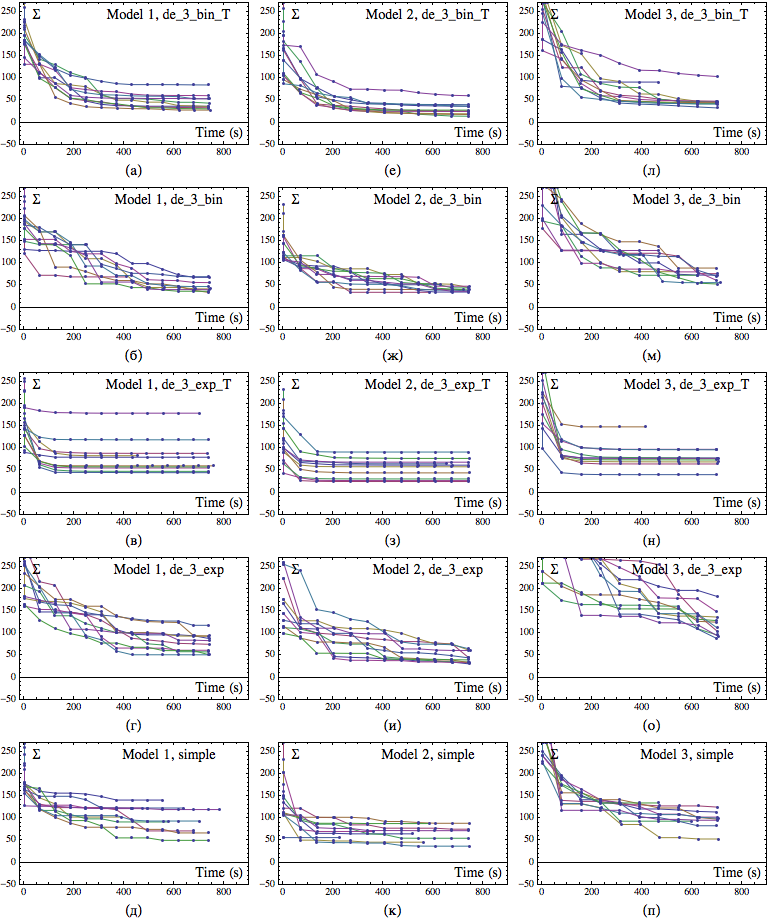
\includegraphics[width=17cm]{recombination}}
  \caption{Графики сходимости метода при различных значениях параметра, 
  отвечающего за способ рекомбинации}
  \label{img:recombination}
\end{figure}


\clearpage
%%%%%%%%%%%%%%%%%%%%%%%%%%%%%%%%%%%%%%%%%%%%%%%%%%%%%%%%%%%%%%%%%%%%%%%%%%%%%%%%
%%%%%%%%%%%%%%%%%%%%%%%%%%%%%%%%%%%%%%%%%%%%%%%%%%%%%%%%%%%%%%%%%%%%%%%%%%%%%%%%
\section{Выводы} \label{s4}

Исходя из численных экспериментов можно сделать несколько выводов:

\begin{enumerate}
  \item Алгоритм ППРЭ хорошо решает поставленную задачу поиска глобального 
  минимума. При этом с биологической точки зрения отличий в поведении системы 
  при использовании найденных параметров нет.
  В результате расчетов получено отклонение модельных концентраций от 
  экспериментальных для первой модели: 0.207112, для второй модели: 0.131785, 
  для третьей модели: 0.102499. 
  За отклонение здесь принимается средняя нормированная сумма квадратов
  разностей, представленная в таблице \ref{contable1}.
  \item Для данных генных сетей набор параметров обширен, по этой причине 
  существует много вариантов их значений, в которых, возможно, достигается 
  глобальный минимум. Соответственно, если в рамках задачи стоит вопрос поиска 
  конкретного вектора параметров, метод ППРЭ, вероятно, не даст 
  удовлетворительных результатов. Однако, такая задача не может встретиться 
  на практике при решении проблемы обратной инженерии генных сетей.
\end{enumerate}

\clearpage
%%%%%%%%%%%%%%%%%%%%%%%%%%%%%%%%%%%%%%%%%%%%%%%%%%%%%%%%%%%%%%%%%%%%%%%%%%%%%%%%
